\begin{document}
	\section{Положение d-металлов в Периодической системе. Электронная конфигурация переходных металлов. Три ряда переходных металлов. Особенности металлов первого переходного ряда, химические свойства их соединений.}
	Переходными называют те элементы у которых частично заполнены d или f оболочки.	Переходные они потому что в таблице они находятся между p и s элементами.
	\begin{figure}[H]
		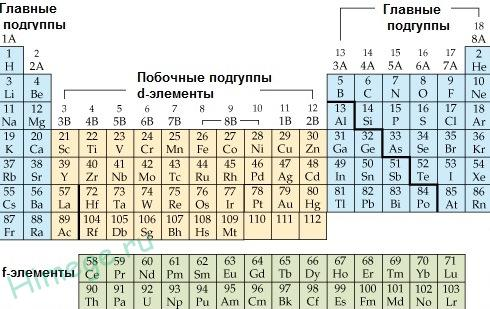
\includegraphics[scale=0.8]{252}
	\end{figure}
	Они имеют низкую энергию ионизации атома и поэтому являются металлами. В расширенной таблице они находятся посередине. Конфигурации уровней вот:
	\begin{figure}[H]
		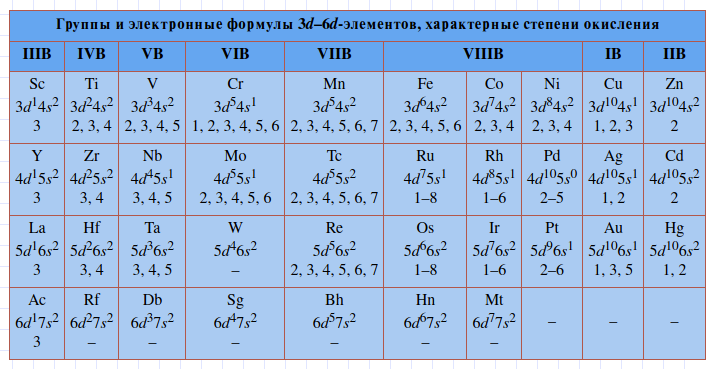
\includegraphics[scale=0.7]{251}
	\end{figure}
Иногда подгруппы называют с указанием верхнего элемента. Например подгруппа меди и тд.

Иногда VIIIB элементы первого ряда называют триадой железа, а второго и третьего платиновыми металлами. 

В каждом ряду конфигурация меняется от $(n- 1)d^1 n s^2 $ до $(n- 1)d^{10} n s^2 $ В середине и особенно конце случаются "проскоки" когда один или два электрона переходят с s уровня в d. Группа цинка особенно устойчива, потому что у нее полностью заполненный уровень. 

Перекрытие орбиталей d уровня частично объясняет прочность и тугоплавкость этих металлов. 
\subsection{Свойства 3d металлов (1 ряд)}
Все это в развернутом варианте есть в Еремине  стр 191


Все они кроме меди расположены в ряду напряжений левее водорода  и потому хорошо растворяются в кислотах 
\begin{align*}
\ce{Fe  + 2 HCl -> FeCl_2 + H_2 \uparrow}
\end{align*}
Они реагируют при нагревании с самыми активными неметаллами: кислородом и галогенами
\begin{align*}
\ce{4Cr +3O_2 -> 2 Cr_2 O_3}
\end{align*}
С менее активными неметаллами: серой, фосфором, углеродом они образуют необычные соединения
\begin{align*}
\ce{Mn + 4P -> MnP_4}
\end{align*}
Все 3d металлы получают восстановлением из оксидов водородом, углеродом или активными металлами
\begin{align*}
\ce{Ti  O_2 + 2Mg -> Ti + 2Mg O}
\end{align*}
В низших степенях окисления они проявляют свойства восстановителей, в высших окислителей
\begin{align*}
4 \mathrm{CuCl}+\mathrm{O}_{2}+4 \mathrm{HCl}=4 \mathrm{CuCl}_{2}+2 \mathrm{H}_{2} \mathrm{O} \quad\left(\mathrm{Cu}^{+1}-\mathrm{e} \rightarrow \mathrm{Cu}^{+2}\right)\\
2 \mathrm{KMnO}_{4}+10 \mathrm{KI}+8 \mathrm{H}_{2} \mathrm{SO}_{4}=2 \mathrm{MnSO}_{4}+5 \mathrm{I}_{2}+6 \mathrm{K}_{2} \mathrm{SO}_{4}+8 \mathrm{H}_{2} \mathrm{O} \\
\left(\mathrm{Mn}^{+7}+5 \mathrm{e} \rightarrow \mathrm{Mn}^{+2}\right)	
\end{align*}
\end{document}